\newpage
\subsection{Funktionen Aufstellen}

2.
Die nebenstehende Kurve veranschaulicht die Wurfparabel eines vom Punkt A
rückgespielten Tennisballs. Der Abschusspunkt liegt 6m vor dem Netz in Höhe
von 0,60m. Der Ball überfliegt das Netz in einer Höhe von 1,20m (B) und trifft
6,00m hinter dem Netz den Boden (C).\\

\begin{itemize}
    \item (a) Man berechne die Funktionsgleichung der Wurfparabel.
    \item (b) Welche Höhe erreicht der Ball 2m nachdem er das Netz passiert hat.
    \item (c) Wo hat der Ball eine Höhe von 80cm?
\end{itemize}

\hfill \break


Angegebene Punkte:
\begin{itemize}
    \item $A = (-6|0.6)$
    \item $A = (0|1.2)$
    \item $A = (0|0)$
\end{itemize}

\hfill \break

Eingesetzt in die Glichung $f(x)=a*x^2+b*x+c$:
\begin{enumerate}
    \item $0.6 = 36a-6b+c$
    \item $1.2 = 0a+0b+c$
    \item $0 = 36a+6b+c$
\end{enumerate}

\hfill \break

A:
$\left(\begin{array}{ccccc}
            36 & -6 & 1 & 0.6 \\
            0  & 0  & 1 & 1.2 \\
            36 & 6  & 1 & 0   \\
        \end{array}\right)$\\

\hfill \break

Ergebnis der Matrix Rechnung:
\begin{itemize}
    \item $a = -0.025$
    \item $b = -0.05$
    \item $c = 1.2$
\end{itemize}

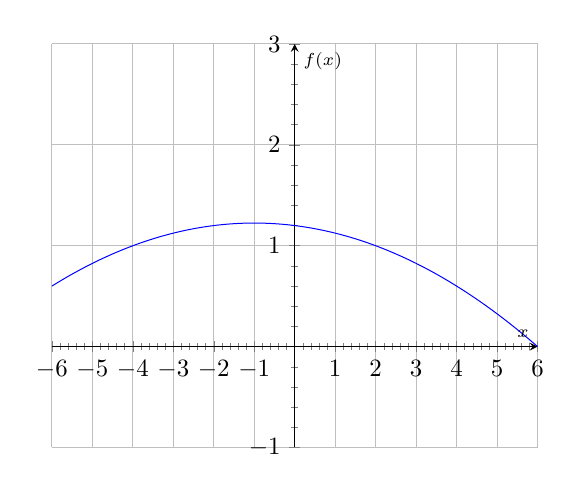
\begin{tikzpicture}[scale=0.9]
    \begin{axis}%
        [
            grid=major,
            xtick={-7,-6,...,7},
            minor x tick num=4, % 4 minor ticks => 5 subintervals
            xmin=-6,
            xmax=6,
            xlabel={\scriptsize $x$},
            axis x line=middle,
            ytick={-5,-4,...,3},
            minor y tick num=4,  % 4 minor ticks => 5 subintervals
            ymin=-1,
            ymax=3,
            ylabel={\scriptsize $f(x)$},
            axis y line=middle,
            no markers,
            samples=100,
            domain=-6:6,
        ]
        \addplot (x,{-0.025*x^2-0.05*x+1.2});
    \end{axis}
\end{tikzpicture}


\subsubsection{Lösung der Aufgabe A}
Die Funktionsgleichung wurden ermittelt in dem die Ergebnisse der Matrix in die Gleichung $f(x)=a*x^2+b*x+c$ Eingesetzt wurden.\\
Die Funktionsgleichung Lauted: $f(x)=-0.025x^2-0.05x+1.2$
\subsubsection{Lösung der Aufgabe B}
Bei dieser Aufgabe muss man den gewünschten Wert (in diesem Fall $2$) in die Funktionsgleichung die bei Beispiel $A$ errechnet wurde einsetzten.
Das Ergebnis lauted $1$
\subsubsection{Lösung der Aufgabe C}
Bei dieser Aufgabe werden die 80cm in Meter umgerechnet und als Ergebnis der Gleichung angegeben so, das $0.8 = -0.025x^2-0.05x+1.2$ entseht.
Danach muss die Gleichung durch eine Division durch $0.8$ noch auf die Form "0 = " gebracht werdendamit Man dei ABC-Formel anwenden kann.\\
die Ergebnisse lauten:
\begin{itemize}
    \item $x_1 = 3.12$
    \item $x_2 = 5.12$
\end{itemize}